% BE_Project.tex
% Do Different Ways of Measuring Greenwashing Agree? A Review of Reality Anchors in Greenwashing Detection
% Compile:  latexmk -pdf BE_Project.tex     (or pdflatex + bibtex + pdflatex x2)
% Bibliography: references.bib (generated from verified Crossref metadata; see papers/SOURCES.md)

\documentclass[12pt,a4paper]{article}

\usepackage[T1]{fontenc}
\usepackage[utf8]{inputenc}
\usepackage{lmodern}
\usepackage[margin=1in]{geometry}
\usepackage{microtype}
\usepackage{amsmath}
\usepackage{booktabs}
\usepackage{longtable}
\usepackage{tabularx}
\usepackage{array}
\usepackage{enumitem}
\usepackage{xcolor}
\usepackage{tikz}
\usetikzlibrary{positioning,arrows.meta,fit,calc}
\usepackage[authoryear,round]{natbib}
\usepackage[hypertexnames=false,colorlinks=true,linkcolor=blue!50!black,citecolor=blue!50!black,urlcolor=blue!50!black]{hyperref}
\usepackage{url}

\setlist{itemsep=2pt,topsep=4pt}
\setlength{\parskip}{5pt}
\setlength{\parindent}{0pt}
\setcounter{tocdepth}{2}
\setcounter{secnumdepth}{3}
\renewcommand{\arraystretch}{1.15}

% ---- small helpers ---------------------------------------------------------
\newcommand{\dg}{$^{\dagger}$}          % marks a detail taken from the research brief, not confirmed from the paper
\newcommand{\fullref}[1]{\par\noindent{\small\textit{Full reference:} #1}\par\smallskip}
\newcommand{\lab}[1]{\textbf{#1}}
\newcommand{\GSI}[1]{GSI-#1}
\newcommand{\co}{CO$_2$e}
\newcolumntype{L}[1]{>{\raggedright\arraybackslash}p{#1}}

\hypersetup{pdftitle={Do Different Ways of Measuring Greenwashing Agree? A Review of Reality Anchors in Greenwashing Detection},
            pdfauthor={Daksha Mehta}}

\begin{document}

% ============================ TITLE PAGE ====================================
\begin{titlepage}
\centering
\vspace*{2.2cm}
{\LARGE\bfseries Do Different Ways of Measuring Greenwashing Agree?\par}
\vspace{0.4cm}
{\Large A Review of Reality Anchors in Greenwashing Detection\par}
\vspace{2.0cm}
{\large Business Economics Project\par}
\vspace{1.6cm}
{\Large\bfseries Daksha Mehta\par}
\vspace{0.4cm}
{\large B.Tech Information Technology\par}
{\large ABV-IIITM Gwalior\par}
\vspace{1.6cm}
{\large Course instructor: \underline{\hspace{6cm}}\par}
{\small\itshape (instructor's name to be added)\par}
\vspace{1.6cm}
{\large November 2026\par}
\vfill
{\small A literature review and research design. No data has been collected and nothing has been
measured.\par}
\end{titlepage}

% ============================ ABSTRACT ======================================
\pagenumbering{roman}
\begin{abstract}
\noindent
Greenwashing is the gap between how environmentally responsible a company says it is and how it
actually behaves. Measuring that gap needs an outside reference, which we call a reality anchor:
regulatory violations, measured emissions, a commercial ratings gap, news and controversies, or
nothing beyond the company's own text. This report reviews 24 papers, five in detail and nineteen
more from four publishers, to ask whether measures built on different anchors identify the same
companies. The talk--action gap appears under every anchor that has been tested. Conclusions on
mandatory disclosure, on who talks more and on whether large firms are cleaner depend on the
measure used, and size and visibility appear to shape what gets measured. As far as we found, no
study builds several greenwashing indices on the same firms, each with a different anchor, and
tests whether they rank the same firms as worst. We set out a design for that test, seven
hypotheses and twelve proposed improvements. This is a review and design project: no data has
been collected and nothing has been measured.
\end{abstract}

\tableofcontents
\clearpage
\listoftables
\clearpage
\pagenumbering{arabic}
% ============================ 1. INTRODUCTION ===============================
\section{Introduction}

\subsection{What greenwashing is}

Companies say a great deal about how green they are, and some of them overstate it. The word for
that is \emph{greenwashing}: making a company look more environmentally responsible than it
really is. In the research we review, it is defined as the gap between two things: what a company
says, in its sustainability report, its press releases and its public commitments; and what it
does, in its actual emissions, its pollution fines and its day-to-day operations
\citep{dorfleitner2024}. If the talk is much better than the actions, that is greenwashing.

The term dates from the 1980s and first covered misleading environmental advertising. Modern
research extends it to sustainability reporting, and across all three pillars of ESG
(environmental, social and governance), not only the environmental one \citep{davidescu2026}. Two
strategies are worth separating: \emph{selective disclosure}, which means staying quiet about
what went badly, and \emph{expressive manipulation}, which means dressing up what is reported in
vague, aspirational language \citep{wang2025}.

\subsection{Why it is hard to measure}

To catch greenwashing automatically we need both halves of the gap as numbers. The talk half is
reasonably straightforward: a computer can score the language of a sustainability report. The
other half is the hard part. What counts as the truth about a company's environmental behaviour?
A field review of 97 articles finds that the research defines and measures greenwashing in
inconsistent ways \citep{forliano2025}, which is the starting point of this project.

\subsection{The reality-anchor idea}

Throughout this report we call the choice of outside reference the \emph{reality anchor}: the
external, non-textual fact against which a greenwashing measure is checked. Published research
uses several, and Table~\ref{tab:anchors} lists them. Two of them, the ratings gap and
controversy, only became visible as separate types once we read the second set of papers.

\begin{table}[!htbp]
\centering
\caption{Reality anchors found in the literature.}
\label{tab:anchors}
\small
\begin{tabularx}{\textwidth}{@{}L{3.1cm}X@{}}
\toprule
\textbf{Reality anchor} & \textbf{What it means}\\
\midrule
Violations & Has a regulator fined the company or found it non-compliant? \\
Emissions / pollution & How much does the company actually emit, as measured? \\
Ratings gap & A commercial disclosure score minus a commercial performance score. \\
Controversy / news events & Which specific negative events has the press reported about the company? \\
Average media tone & How negative or positive is press coverage about the company on average? \\
None (text-internal) & The report's language is analysed without checking it against anything. \\
\bottomrule
\end{tabularx}
\end{table}

\subsection{Research question}

The question behind the project is whether published greenwashing measures, built on different
anchors, identify the same companies. Our primary version of it is:

\begin{quote}
\emph{Do greenwashing measures built on media sentiment identify the same firms as measures built
on regulatory violation records, or is media-anchored greenwashing detection largely measuring
firm visibility?}
\end{quote}

The matters it raises are practical. ESG ratings influence index inclusion, fund mandates and the
cost of capital. If the tools built to detect greenwashing reward visibility and polished writing
rather than conduct, they reproduce the problem they were built to expose.

\subsection{Contribution}

This report makes four contributions. First, it sorts 24 papers by reality anchor and shows how
the anchor choice organises an otherwise scattered literature. Second, it explains three apparent
contradictions in the literature by the choice of measure (Section~\ref{sec:shows}). Third, it
states the gap more precisely than we first did, after finding that some papers come close to what
we propose (Section~\ref{sec:gap}). Fourth, it sets out a design and twelve improvements for
testing the gap, including three new hypotheses (Sections~\ref{sec:design} and
\ref{sec:combining}).

\textbf{Scope.} This is a literature review and research design. We have not written analysis code,
scrapers or models, have not implemented any paper, and have not retrieved any data. Every
statement about what a paper found is a statement about that paper. Statements about what we
\emph{would} do are proposals. Section~\ref{sec:threats} says which papers we read in full and which
only by abstract.

% ============================ 2. THE ORIGINAL FIVE ==========================
\section{The original five papers}
\label{sec:five}

The first five papers gave us the reality-anchor idea. We summarise each, with what we understood
and what could be improved.

\subsection{Paper 1: the Greenwashing Severity Index}

\fullref{Davidescu, A. A., Manta, E. M., B{\^\i}rlan, I., Miler, A. M., \& Ni{\c t}{\u a}, S. C. (2026).
Detecting greenwashing in ESG disclosure: An NLP-based analysis of Central and Eastern European
firms. \textit{Sustainability, 18}(3), 1486. \url{https://doi.org/10.3390/su18031486}}

\citet{davidescu2026} take 204 large companies in Central and Eastern Europe, collect their
sustainability reports and news coverage, and build a Greenwashing Severity Index (GSI). They
describe it as measuring the gap between what a company says about itself and what the press says
about it.

\lab{What they did.} The method is dictionary-based. The authors built four word lists by hand: a
greenwashing list of 1,140 ``good'' words and 990 ``bad'' words, and separate 122-word lists for
Environmental, Social and Governance terms. They count the words, weight them with TF--IDF (a
technique that boosts words distinctive to one document and plays down words that appear
everywhere), and combine them into one number per company. The average GSI was 0.5765, which they
read as moderate greenwashing everywhere. Germany scored worst (0.6086) and Lithuania best
(0.5157). Finance, online commerce and aviation were the worst industries and construction the
best. Large companies scored better (0.49), which the authors attribute to closer scrutiny.

\lab{The formula finding.} Working through the formula, we found that it reduces to
\begin{equation}
\mathrm{GSI} = \tfrac13\,E_{\mathrm{tfidf}} + \tfrac13\,S_{\mathrm{tfidf}} + \tfrac13\,G_{\mathrm{tfidf}},
\end{equation}
and that all three inputs are calculated from the company's own report. The news articles the
authors collected never enter it. So although the paper says the GSI measures the gap between
what a company claims and how the press describes it, the published formula measures no such
gap: it measures how densely a report is packed with ESG vocabulary. We checked this by
recalculating the authors' own published figures (Table~\ref{tab:gsiverify}). The equal-weighted
mean of the three published component scores reproduces the published GSI to four decimal places.

\begin{table}[!htbp]
\centering
\caption{Verification of the Paper 1 aggregation rule against the paper's own published figures
\citep{davidescu2026}. Lithuania differs by 0.0001, consistent with rounding of the inputs.}
\label{tab:gsiverify}
\small
\begin{tabular}{@{}lccccc@{}}
\toprule
Group & E washing & S washing & G washing & Mean of the three & Published GSI \\
\midrule
Whole sample & 0.4474 & 0.6566 & 0.6254 & 0.5765 & 0.5765 \\
Germany      & 0.5061 & 0.6602 & 0.6595 & 0.6086 & 0.6086 \\
Poland       & 0.4203 & 0.6185 & 0.5853 & 0.5414 & 0.5414 \\
Lithuania    & 0.3880 & 0.5953 & 0.5636 & 0.5156 & 0.5157 \\
\bottomrule
\end{tabular}
\end{table}

\lab{What could be improved.} Several other things did not hold up when we checked them. The main
claim that firms emphasising one ESG pillar over the others show ``significantly higher''
greenwashing is not significant on the paper's own tests ($p=0.077$ and $p=0.064$, both with
confidence intervals that include zero). The text says all GSI values exceed 0.5, but the paper's
own table reports a minimum of 0.00063. The word-scoring scale is described in two contradictory
ways ($-1$ to $+1$ in one section, $-3$ to $+3$ in another). Topic modelling is described, but no
topic-model result appears in the index or the tables. We therefore treat the GSI as the formula
as published, and not as a validated instrument. The journal is peer-reviewed and indexed, but the Norwegian
and Finnish publication-quality lists do not credit it, and the problems above are consistent with
limited review scrutiny (see \texttt{papers/SOURCES.md}).

\subsection{Paper 2: violations as the anchor}

\fullref{Gorovaia, N., \& Makrominas, M. (2025). Identifying greenwashing in corporate-social
responsibility reports using natural-language processing. \textit{European Financial Management,
31}(1), 427--462. \url{https://doi.org/10.1111/eufm.12509}}

\citet{gorovaia2025} split US companies by a hard external fact, whether the company has been
fined for an environmental violation, and then read both groups' sustainability reports.

\lab{What they did.} Rather than collecting whichever reports were easy to find, which would
over-select large, green, well-organised firms, they started from the full population of firms,
matched each violator to a similar non-violator by propensity score, and only then looked for
reports. The result is 993 matched pairs, 1,120 reports and 441 companies over 2008 to 2022.

\lab{Key findings.} Violators write longer reports (20,304 words against 15,091), more
positively (0.823 against 0.816), and with more environmental content (0.185 against 0.175);
their text is less readable, though that difference alone is not significant in the univariate
comparison. A staggered difference-in-differences test shows that firms change their reporting
after a violation: environmental content rises by 0.175 ($p<0.001$). This is the closest thing in
the first five papers to catching greenwashing as it happens.

\lab{What could be improved.} A fine proves a violation, but the absence of a fine does not prove
clean conduct, and the authors say so. Their violation data come from commercial databases
(MSCI, Refinitiv) rather than the regulator directly, which our design would change.

\subsection{Paper 3: emissions as the anchor}

\fullref{Peng, X., Li, J., Tang, Q., Lan, Y.-C., \& Cui, X. (2024). Do environmental scores
become multinational corporations' strategic ``greenwashing'' tool for window-dressing carbon
reduction? A cross-cultural analysis. \textit{Business Strategy and the Environment, 33}(3),
2084--2115. \url{https://doi.org/10.1002/bse.3586}}

\citet{peng2024} use no text analysis. They check the environmental score that a rating agency
gives to large companies against how much carbon those companies actually emit: 199 Fortune Global
500 firms in 27 countries, 2001--2020.

\lab{Key findings.} Higher environmental scores go with higher emissions, not lower: the
coefficient is 0.775 for next-year absolute emissions and 1.304 for emissions per unit of sales,
both significant at the 1\% level. Mandatory disclosure did not close the gap; the effect is if
anything larger where disclosure is mandatory (1.532 against 0.510). The Paris Agreement did not
prevent it either, and in high power-distance societies it grew worse afterwards. This shows
that the reality-check approach works with a completely different method from Paper 2, and reaches
the same conclusion.

\lab{What could be improved.} The scores come from a single provider; the culture measures are
static over twenty years; and financial firms are excluded.

\subsection{Paper 4: a deep-learning index with no external anchor}

\fullref{Wang, X., Gao, X., \& Sun, M. (2025). Construction and analysis of corporate greenwashing
index: a deep learning approach. \textit{EPJ Data Science, 14}(1), 44.
\url{https://doi.org/10.1140/epjds/s13688-025-00562-w}}

\citet{wang2025} use MacBERT, a modern language model, to read Chinese company reports sentence
by sentence and score greenwashing for 9,534 company-years from 2008 to 2023.

\lab{What they did.} They split greenwashing into selective disclosure (the share of required
topics the company never mentions) and expressive manipulation (the share of statements that are
vague and aspirational rather than concrete and checkable). A statement is substantive if it can
be checked and would be hard to fake, and symbolic if it is only aspiration, vague description or
repeated wording. The two components are combined by a geometric mean, so a company scores badly
overall only if it does both. The model agrees with human labellers 97.79\% of the time on the
first component and 95.13\% on the second.

\lab{Why a language model.} A keyword list cannot tell a real commitment from a vague aspiration,
because both use the same words. ``We are committed to reducing emissions'' and ``we reduced
emissions by 12\% in 2023'' share most of their vocabulary. This is effectively a criticism of
Paper 1's approach.

\lab{What could be improved.} The index is never checked against reality: both components come
from the report's own text, so the 97.79\% figure means the model agrees with human readers, not
that the company pollutes less. The authors do not claim otherwise. The sample is Chinese A-share
firms under one disclosure regime.

\subsection{Paper 5: a map of the research landscape}

\fullref{Forliano, C., Battisti, E., de Bernardi, P., \& Kliestik, T. (2025). Mapping the
greenwashing research landscape: a theoretical and field analysis. \textit{Review of Managerial
Science, 19}(11), 3407--3456. \url{https://doi.org/10.1007/s11846-025-00856-3}}

\citet{forliano2025} is a systematic review of 97 peer-reviewed articles. The field splits into
four themes: symbolic management and CSR communication; environmental regulation and institutional
complexity; performance and sustainable practices; and marketing, perception and trust. Research
is dominated by macro-level theories (legitimacy, institutional and stakeholder theory), and the
authors propose organising the field across macro, meso and micro levels.

It is moderately useful for us. It maps theories rather than measurement methods, so it does not
compare violation-based, media-based and emissions-based approaches, and its coverage closed in
February 2025, before Papers 1 and 4 appeared. It does confirm that the field defines and measures
greenwashing in inconsistent ways.
% ============================ 3. EXTENDED LITERATURE ========================
\section{The extended literature}
\label{sec:ext}

Nineteen more papers, from four publishers (Elsevier, Springer, Emerald and Taylor \& Francis),
test the reality-anchor idea from different angles. We group them into six themes. For each paper
we give the full reference, what the authors did, the key finding, the reality anchor and how it
helps the project.

\textbf{How much of each paper we read.} We read four of the nineteen in full (Bingler et al.\ 2022;
Luu et al.\ 2025; Dorfleitner \& Utz 2024; Raghunandan \& Rajgopal 2022), because they are legally
open access and we could download them. For the other fifteen we read the abstract and publisher
metadata. A dagger (\dg) marks a detail that comes from our research brief and that the abstract
or paper we read does not confirm. Section~\ref{sec:threats} gives the full account.

\subsection{Group A: measuring the ``talk'' side}

\subsubsection*{Lagasio (2024): the ESG-washing Severity Index}
\fullref{Lagasio, V. (2024). ESG-washing detection in corporate sustainability reports.
\textit{International Review of Financial Analysis, 96}, 103742.
\url{https://doi.org/10.1016/j.irfa.2024.103742} (Elsevier)}
\lab{What they did.} \citet{lagasio2024} build an ESG-washing Severity Index (ESGSI) for 749
listed companies by combining sentiment analysis with the frequency of sustainability terms in
their reports. \lab{Finding.} The index varies markedly across industries and regions. \lab{Anchor.}
None in substance, as far as the abstract shows: both ingredients come from the same report.
\lab{For us.} It is the closest relative of Paper 1. We found that Paper 1 does not cite it. Whether
the ESGSI formula has any external term, and so whether our Paper 1 finding applies to a family of
``severity indices'', is an open question that needs the full text. We do not state it as a finding.

\subsubsection*{Bingler et al.\ (2024): cheap talk, initiatives, emissions and reputation}
\fullref{Bingler, J. A., Kraus, M., Leippold, M., \& Webersinke, N. (2024). How cheap talk in
climate disclosures relates to climate initiatives, corporate emissions, and reputation risk.
\textit{Journal of Banking \& Finance, 164}, 107191. \url{https://doi.org/10.1016/j.jbankfin.2024.107191}
(Elsevier)}
\lab{What they did.} \citet{bingler2024} introduce ClimateBert CTI, a deep-learning model that
flags climate-related ``cheap talk'' (imprecise, non-committal statements) in the annual reports
of MSCI World firms. The sample is 14,584 annual reports from 2010 to 2020\dg. \lab{Finding.}
Only targeted climate engagement is associated with less cheap talk, and voluntary climate
disclosures are associated with more. Cheap talk correlates with more negative news coverage and
higher emissions growth. \lab{Anchor.} One talk measure, related to emissions and news separately.
\lab{For us.} This is the most important new paper. It is a published way to measure the talk side
(the share of imprecise versus precise commitments\dg). It also narrows our gap, because it touches
two anchors; but it treats them as separate correlates rather than as competing greenwashing
measures whose rankings are compared (Section~\ref{sec:gap}).

\subsubsection*{Bingler et al.\ (2022): ClimateBert on TCFD disclosures}
\fullref{Bingler, J. A., Kraus, M., Leippold, M., \& Webersinke, N. (2022). Cheap talk and
cherry-picking: What ClimateBert has to say on corporate climate risk disclosures. \textit{Finance
Research Letters, 47}, 102776. \url{https://doi.org/10.1016/j.frl.2022.102776} (Elsevier). Full text read.}
\lab{What they did.} \citet{bingler2022} fine-tune ClimateBERT on more than 17,300 hand-labelled
sentences for the four TCFD categories and more than 300,000 general sentences, then apply it to
the annual reports of 818 firms that support the TCFD, fiscal years 2014--2019. \lab{Finding.} The
firms' support is mostly cheap talk, and firms cherry-pick, reporting mainly non-material
information. The authors find no considerable increase in reporting after 2016, when EU
non-financial reporting rules began to apply. \lab{Anchor.} None; the analysis is text-internal.
\lab{For us.} Voluntary framework membership is not a sign of honest conduct, which supports our
argument against treating disclosure volume as a proxy for it. Note that the DOI in our brief was
wrong by one year; the corrected DOI is the one above.

\subsubsection*{Hrasky (2012): symbolism or action in carbon-footprint disclosure}
\fullref{Hrasky, S. (2012). Carbon footprints and legitimation strategies: symbolism or action?
\textit{Accounting, Auditing \& Accountability Journal, 25}(1), 174--198.
\url{https://doi.org/10.1108/09513571211191798} (Emerald)}
\lab{What they did.} \citet{hrasky2012} content-analyse the sustainability and annual reports of the
ASX Top 50 companies, comparing 2008 with 2005, and classify carbon-footprint disclosure as action
or symbolism, by more and less carbon-intensive sector. \lab{Finding.} Disclosure rates are rising.
Carbon-intensive sectors appear to pursue a moral legitimation strategy underpinned by substantive
action, while less intensive sectors rely more on symbolic disclosure. \lab{Anchor.} Sector carbon
intensity, a coarse stand-in for emissions. \lab{For us.} It is an early manual version of the
symbolic--substantive split that Paper 4 automates. It also suggests that symbolic talk sits in
low-emission sectors, which supports sector fixed effects and checking whether a talk score behaves
differently by sector.

\subsection{Group B: disclosure against measured performance}

\subsubsection*{Clarkson et al.\ (2008): performance and disclosure}
\fullref{Clarkson, P. M., Li, Y., Richardson, G. D., \& Vasvari, F. P. (2008). Revisiting the
relation between environmental performance and environmental disclosure: An empirical analysis.
\textit{Accounting, Organizations and Society, 33}(4--5), 303--327.
\url{https://doi.org/10.1016/j.aos.2007.05.003} (Elsevier)}
\lab{What they did.} \citet{clarkson2008} study 191 firms from the five most polluting US
industries, using a GRI-based content index of discretionary environmental disclosure\dg.
\lab{Finding.} Better environmental performance is associated with more disclosure, in line with
voluntary disclosure theory, although legitimisation patterns still appear\dg. \lab{Anchor.}
Emissions or pollution performance. \lab{For us.} A classic counterweight to Paper 2: the sign of
the talk--performance relationship depends on what kind of talk is measured, which is why our
design scores verifiable action statements separately from vague commitments. We have no abstract
for this paper, so everything here rests on our brief\dg.

\subsubsection*{Tadros and Magnan (2019): mapping performance into disclosure}
\fullref{Tadros, H., \& Magnan, M. (2019). How does environmental performance map into
environmental disclosure? A look at underlying economic incentives and legitimacy aims.
\textit{Sustainability Accounting, Management and Policy Journal, 10}(1), 62--96.
\url{https://doi.org/10.1108/SAMPJ-05-2018-0125} (Emerald)}
\lab{What they did.} \citet{tadros2019} analyse 78 firms from environmentally sensitive industries
over 14 years, across annual reports, 10-Ks and sustainability reports. \lab{Finding.} High
performers disclose more; economic and legitimacy factors act differently for high and low
performers; and there is little evidence that low performers use disclosure to legitimise.
\lab{Anchor.} Environmental performance (the abstract does not say which measure).
\lab{For us.} It uses 10-Ks alongside sustainability reports, which supports our plan to use SEC
EDGAR text as a supplementary talk source, and it reinforces the reversal of the legitimacy
prediction.

\subsubsection*{Luu et al.\ (2025): the GHGRP as a natural experiment}
\fullref{Luu, N. H., Le, C., Luu, H. N., \& Nguyen, D. T. K. (2025). Does mandatory greenhouse gas
emissions reporting program deter corporate greenwashing? \textit{Journal of Environmental
Management, 373}, 123740. \url{https://doi.org/10.1016/j.jenvman.2024.123740} (Elsevier). Full text read.}
\lab{What they did.} \citet{luu2025} use the US EPA Greenhouse Gas Reporting Program (GHGRP) as a
quasi-natural experiment with a difference-in-differences design. From 2010, facilities emitting
more than 25,000 metric tons of greenhouse gas a year must report. The sample is 2,731 listed US
firms, 2007--2022, of which 134 are treated and 2,597 are controls. Greenwashing is a ratings gap:
the standardised Refinitiv ESG disclosure score minus the standardised Refinitiv ESG performance
score, adopted from \citet{yu2020}. \lab{Finding.} Greenwashing falls after the GHGRP: in the fullest
specification by about 30.74\% of the sample mean (0.537 against 1.747). The programme pushes firms
to improve actual ESG performance while curbing inflated claims, and larger, more profitable
firms show the largest falls. \lab{Anchor.} A ratings gap, with the GHGRP as the policy shock.
Both halves of the gap come from one vendor. \lab{For us.} It uses our planned emissions source in
the same country and period, gives us a ready test (H7), and it contradicts Paper 3 on whether
mandatory disclosure helps (Section~\ref{sec:shows}).

\subsubsection*{Cho et al.\ (2015): the more things change}
\fullref{Cho, C. H., Michelon, G., Patten, D. M., \& Roberts, R. W. (2015). CSR disclosure: the
more things change\ldots? \textit{Accounting, Auditing \& Accountability Journal, 28}(1), 14--35.
\url{https://doi.org/10.1108/AAAJ-12-2013-1549} (Emerald)}
\lab{What they did.} \citet{cho2015} compare Fortune 500 CSR disclosure from the late 1970s with
2010 and test whether the market values it. \lab{Finding.} Disclosure breadth rose
significantly, but the relationship between legitimacy factors and disclosure did not change, and
CSR disclosure is not positively valued by investors. \lab{Anchor.} None directly; legitimacy and
exposure factors. \lab{For us.} Three decades of evidence that disclosure tracks exposure and
visibility, which is the mechanism behind our salience hypothesis.

\subsection{Group C: the ratings-gap anchor}

\subsubsection*{Yu, Luu and Chen (2020): greenwashing in ESG disclosures}
\fullref{Yu, E. P., Luu, B. V., \& Chen, C. H. (2020). Greenwashing in environmental, social and
governance disclosures. \textit{Research in International Business and Finance, 52}, 101192.
\url{https://doi.org/10.1016/j.ribaf.2020.101192} (Elsevier)}
\lab{What they did.} \citet{yu2020} define greenwashers as firms that look very transparent and
disclose large quantities of ESG data but perform poorly\dg. They build peer-relative greenwashing
scores for 1,925 large-cap firms across countries\dg. We can confirm the structure of the measure
from two papers we read in full: it is the standardised disclosure score minus the standardised
performance score \citep{luu2025}, described as a relative index based on the disconnection between
disclosure and performance \citep{wang2025}. \lab{Finding.} Scrutiny from independent directors,
institutional investors, a less corrupt country system and cross-listing deters greenwashing\dg.
\lab{Anchor.} Ratings gap. \lab{For us.} It is the template that later papers copy. We propose
adding it as a fourth index, because it is what applied finance actually uses, and its peer-relative
standardisation is a good model for standardising our own indices. We have no abstract for this
paper, so the description above rests on our brief\dg\ plus the two papers cited.

\subsubsection*{Liu et al.\ (2024): crash risk}
\fullref{Liu, G., Qian, H., Shi, Y., Zhang, Y., \& Wu, F. (2024). Does ESG report greenwashing
increase stock price crash risk? \textit{China Journal of Accounting Studies, 12}(3), 615--639.
\url{https://doi.org/10.1080/21697213.2024.2303070} (Taylor \& Francis)}
\lab{What they did.} \citet{liu2024} ask whether ESG report greenwashing raises the risk of a
stock price crash, using Chinese listed firms, 2014--2021, and the disclosure-minus-performance
measure of \citet{yu2020}\dg. \lab{Finding.} Greenwashing raises crash risk, through greater
information asymmetry; the effect is stronger under voluntary disclosure and in private
enterprises, and good governance suppresses it. \lab{Anchor.} Ratings gap\dg. \lab{For us.} It shows
that a greenwashing measure can be validated against a future market outcome, which suggests a
tie-breaker: whichever index best predicts later outcomes has the stronger claim to measure
something real (H6).

\subsubsection*{Dorfleitner and Utz (2024): a conceptual framework}
\fullref{Dorfleitner, G., \& Utz, S. (2024). Green, green, it's green they say: a conceptual
framework for measuring greenwashing on firm level. \textit{Review of Managerial Science, 18}(12),
3463--3486. \url{https://doi.org/10.1007/s11846-023-00718-w} (Springer). Full text read.}
\lab{What they did.} \citet{dorfleitner2024} propose a firm-level greenwashing indicator equal to
apparent minus real green performance in each of several dimensions of greenness, built from five
pillars of information: soft ESG data, textual self-representation, green marketing expenses and
green virtue (the apparent side), and hard ESG data (the real side). Where real performance is hard
to measure, it is approximated from evident misconduct (for example a controversy score), so that
the indicator becomes apparent performance times misconduct. Weights can be calibrated on firm-years
where case examination shows whether greenwashing occurred. A two-firm illustration with Refinitiv
2022 data gives indicator values of 0.136 for Delivery Hero and 0.909 for Zalando.
\lab{Finding.} A framework, not an empirical result; the authors read the misconduct version as a
measure of greenwashing risk rather than of disclosed greenwashing. \lab{Anchor.} Multiple,
combined. \lab{For us.} It is the only paper that explicitly proposes combining several sources into
one indicator, and so the backbone of our combining section. The empirical step it does not take
is to test whether the pillars agree before they are combined.

\subsection{Group D: the violations anchor}

\subsubsection*{Raghunandan and Rajgopal (2022): ESG funds}
\fullref{Raghunandan, A., \& Rajgopal, S. (2022). Do ESG funds make stakeholder-friendly
investments? \textit{Review of Accounting Studies, 27}(3), 822--863.
\url{https://doi.org/10.1007/s11142-022-09693-1} (Springer). Full text read.}
\lab{What they did.} \citet{raghunandan2022} compare 147 self-labelled US ESG mutual funds (from 74
asset managers) with 2,428 non-ESG funds at the same institutions, 2010--2018, using Violation
Tracker (a database of violations of federal laws, compiled by the non-profit Good Jobs First) for
compliance records and carbon emissions data. \lab{Finding.} ESG funds hold firms with worse
compliance records for labour and environmental law, higher fines, and higher emissions per unit of
revenue, yet with higher ESG scores. ESG scores are correlated with the quantity of voluntary
disclosure (and, in the text, with news-coverage metrics), but not with compliance records or
actual emissions. \lab{Anchor.} Violations and emissions, compared against ESG scores, at the level
of fund portfolios. \lab{For us.} It is an independent confirmation of the talk--action gap with a
violations anchor; it points to a violations database to cross-check our own aggregation of EPA
facility records (its access terms are unchecked); and it shows that ratings and violations
disagree, a partial version of our own question.

\subsection{Group E: media, controversy and events}

\subsubsection*{Boiral (2013): sustainability reports as simulacra}
\fullref{Boiral, O. (2013). Sustainability reports as simulacra? A counter-account of A and A+ GRI
reports. \textit{Accounting, Auditing \& Accountability Journal, 26}(7), 1036--1071.
\url{https://doi.org/10.1108/AAAJ-04-2012-00998} (Emerald)}
\lab{What they did.} \citet{boiral2013} counter-account 23 GRI A and A+ sustainability reports from
energy and mining firms (about 2,700 pages, organised around 92 GRI indicators) against 116
significant news events about the firms' sustainability problems. \lab{Finding.} Ninety per cent of
the significant negative events were not reported. \lab{Anchor.} Media events, matched by hand.
\lab{For us.} A hand-built media anchor that measures omission rather than tone, and so a better
use of media than an average of tone (Improvement 4).

\subsubsection*{Ghitti et al.\ (2024): the agency of greenwashing}
\fullref{Ghitti, M., Gianfrate, G., \& Palma, L. (2024). The agency of greenwashing.
\textit{Journal of Management and Governance, 28}(3), 905--941.
\url{https://doi.org/10.1007/s10997-023-09683-8} (Springer)}
\lab{What they did.} \citet{ghitti2024} propose a novel set of greenwashing measures and relate
them to board characteristics. \lab{Finding.} Firms with more independent directors tend to
greenwash more, the effect of board size is ambiguous, and greenwashing reduces firm value.
\lab{Anchor.} Our brief says the measure is the gap between the ESG score and the ESG controversy
score, and that it contrasts ex-ante intentions with ex-post outcomes. \textbf{This construction is
unverified:} the abstract says only that the authors propose a novel set of measures, and we could
not read the method section. \lab{For us.} If confirmed, it is a controversy-anchored measure for US
firms\dg, and a second example of validation against a market outcome.

\subsubsection*{Bacher et al.\ (2025): greenwashing risk in asset pricing}
\fullref{Bacher, K., D{\o}skeland, M., Gra{\c c}a, R., Lavrutich, M., Pierce, M., \& Pimentel, R.
(2025). Greenwashing risk in asset pricing: the shift after the Paris agreement. \textit{Quantitative
Finance, 25}(11), 1851--1872. \url{https://doi.org/10.1080/14697688.2025.2563091} (Taylor \& Francis)}
\lab{What they did.} \citet{bacher2025} use double-selection LASSO and a two-pass regression on a
global dataset to test whether greenwashing is a priced asset pricing factor. According to our
brief, the measure is the one from \citet{ghitti2024}\dg. \lab{Finding.} In Europe before the Paris
Agreement (2011--2015), the greenwashing factor is priced and greenwashing firms underperform
genuinely sustainable peers; after Paris it has no significant pricing power. \lab{Anchor.}
Controversy\dg. \lab{For us.} It shows controversy-anchored measures in use in a leading
quantitative finance journal, and echoes the Paris result of Paper 3 from another angle.

\subsubsection*{Utz (2019): corporate scandals}
\fullref{Utz, S. (2019). Corporate scandals and the reliability of ESG assessments: evidence from
an international sample. \textit{Review of Managerial Science, 13}(2), 483--511.
\url{https://doi.org/10.1007/s11846-017-0256-x} (Springer)}
\lab{What they did.} An event study on press releases of corporate scandals, using Asset4 ratings\dg.
\lab{Finding.} Retrospective controversy indicators drop during the scandal period and then
rebound, forward-looking indicators rise slightly, and aggregated ESG assessments are of little use
for predicting scandals\dg. \lab{Anchor.} Media events (scandals), used to test ratings.
\lab{For us.} It provides the method for an event-response test: a measure that claims to capture
misconduct should move when a real scandal or enforcement action becomes public (Improvement 3).
We have no abstract for this paper, so it rests on our brief\dg.

\subsubsection*{Cho (2009): Total SA after Erika and AZF}
\fullref{Cho, C. H. (2009). Legitimation strategies used in response to environmental disaster: A
French case study of Total SA's Erika and AZF incidents. \textit{European Accounting Review,
18}(1), 33--62. \url{https://doi.org/10.1080/09638180802579616} (Taylor \& Francis)}
\lab{What they did.} \citet{cho2009} is a case study of Total after the 1999 Erika oil spill and the
2001 AZF plant explosion, framed within legitimacy theory. \lab{Finding.} Total used disclosure to
legitimise and downplay rather than to account. \lab{Anchor.} Events, at case level. \lab{For us.} It
is the qualitative mechanism behind Paper 2's difference-in-differences result (firms change their
writing after being caught), and helps us interpret any post-event change in a talk score.

\subsection{Group F: reliability of the measures themselves}

\subsubsection*{Drempetic et al.\ (2020): size bias in ESG scores}
\fullref{Drempetic, S., Klein, C., \& Zwergel, B. (2020). The influence of firm size on the ESG
score: Corporate sustainability ratings under review. \textit{Journal of Business Ethics, 167}(2),
333--360. \url{https://doi.org/10.1007/s10551-019-04164-1} (Springer)}
\lab{What they did.} \citet{drempetic2020} examine Asset4 ratings and find that firm size, the
resources available for producing ESG data and data availability all raise a firm's ESG
score\dg, which favours larger firms. A follow-up, \citet{dobrick2023}, reports that the bias persists
in Refinitiv data\dg; we count it as a supplementary reference, not one of the 24 papers.
\lab{Anchor.} Not applicable (a study of rating bias). \lab{For us.} Strong prior evidence for the
salience hypothesis, applied to commercial ratings: if size inflates ratings, it plausibly inflates
media-based and disclosure-based measures too. Our regressions should control for size. We have no
abstract for this paper, so it rests on our brief\dg.

\subsubsection*{Gibson Brandon et al.\ (2021): ESG rating disagreement}
\fullref{Gibson Brandon, R., Krueger, P., \& Schmidt, P. S. (2021). ESG rating disagreement and
stock returns. \textit{Financial Analysts Journal, 77}(4), 104--127.
\url{https://doi.org/10.1080/0015198X.2021.1963186} (Taylor \& Francis)}
\lab{What they did.} \citet{gibsonbrandon2021} take ESG ratings from seven providers for S\&P 500
firms, 2010--2017, and relate rating disagreement to stock returns. \lab{Finding.} Returns are
positively related to disagreement, mainly disagreement about the environmental dimension. Our
brief adds that the average pairwise correlation between providers is about 0.45 and that
disagreement is higher for the largest firms\dg. \lab{Anchor.} Not applicable (it compares raters).
\lab{For us.} It is the methodological model for our study: it does for ESG raters what we propose for
greenwashing anchors, namely measure agreement across measures of the same concept. It also gives a
benchmark for judging our correlations, once the 0.45 figure is confirmed from the paper.

\subsection{Summary of all 24 papers}

Table~\ref{tab:all24} lists all 24. Anchor types are those of Table~\ref{tab:anchors}: V
violations, E emissions or pollution, R ratings gap, C controversy or news events, M average
media tone, N none. A dagger marks a detail taken from our research brief.

{\scriptsize
\setlength{\tabcolsep}{3pt}
\begin{longtable}{@{}L{0.5cm}L{2.2cm}L{1.5cm}L{2.9cm}L{1.3cm}L{2.2cm}L{3.8cm}@{}}
\caption{All 24 papers: author, year, publisher, sample, anchor, method and headline.}\label{tab:all24}\\
\toprule
\textbf{\#} & \textbf{Paper} & \textbf{Publisher} & \textbf{Sample} & \textbf{Anchor} & \textbf{Method} & \textbf{Headline}\\
\midrule
\endfirsthead
\toprule
\textbf{\#} & \textbf{Paper} & \textbf{Publisher} & \textbf{Sample} & \textbf{Anchor} & \textbf{Method} & \textbf{Headline}\\
\midrule
\endhead
\midrule \multicolumn{7}{r}{\emph{continued on next page}}\\
\endfoot
\bottomrule
\endlastfoot
1 & \citet{davidescu2026} & MDPI & 204 CEE firms, 2023 & N (M claimed, not in formula) & Dictionary, TF--IDF & Mean GSI 0.5765; formula has no media term\\
2 & \citet{gorovaia2025} & Wiley & 441 US firms, 2008--2022 & V & Text measures, PSM, DiD & Violators write more and more positively; reporting shifts after a violation\\
3 & \citet{peng2024} & Wiley & 199 Fortune Global 500 firms, 2001--2020 & E & Panel regression & Higher environmental score goes with more emissions\\
4 & \citet{wang2025} & Springer & 9,534 Chinese firm-years, 2008--2023 & N & MacBERT classifiers & Symbolic versus substantive split; 97.79\% agreement with human labels (component 1)\\
5 & \citet{forliano2025} & Springer & 97 articles & n/a & Systematic review & Four themes; macro theories dominate\\
6 & \citet{lagasio2024} & Elsevier & 749 listed firms & N (abstract) & Sentiment plus term frequency & ESGSI varies by industry and region\\
7 & \citet{bingler2024} & Elsevier & MSCI World (14,584 reports, 2010--2020\dg) & N, then E and C separately & ClimateBert CTI & Cheap talk goes with negative news and higher emissions growth\\
8 & \citet{bingler2022} & Elsevier & 818 TCFD supporters, FY2014--2019 & N & ClimateBERT & TCFD support mostly cheap talk; cherry-picking\\
9 & \citet{hrasky2012} & Emerald & ASX Top 50, 2005 and 2008 & E (sector, coarse) & Manual content analysis & Intensive sectors lean on action, others on symbolism\\
10 & \citet{clarkson2008} & Elsevier & 191 US firms, five polluting industries\dg & E & GRI-based index\dg & Better performers disclose more\dg\\
11 & \citet{tadros2019} & Emerald & 78 firms, 14 years & E (measure not in abstract) & Panel regression & High performers disclose more; little legitimising by low performers\\
12 & \citet{luu2025} & Elsevier & 2,731 US firms, 2007--2022 (134 treated) & R, GHGRP as shock & Difference-in-differences & Greenwashing fell after GHGRP (about 31\% of the mean)\\
13 & \citet{cho2015} & Emerald & Fortune 500, late 1970s vs 2010 & None direct & Indices, valuation model & Breadth up; legitimacy link unchanged; not valued by investors\\
14 & \citet{yu2020} & Elsevier & 1,925 large-cap firms\dg & R & Peer-relative gap\dg & Scrutiny deters greenwashing\dg\\
15 & \citet{liu2024} & Taylor \& Francis & Listed firms (Chinese, 2014--2021\dg) & R\dg & Regression & Greenwashing raises crash risk\\
16 & \citet{dorfleitner2024} & Springer & Conceptual, two-firm illustration & Multiple, combined & Framework & Five pillars; misconduct factor\\
17 & \citet{raghunandan2022} & Springer & 147 ESG funds, 74 managers, 2,428 non-ESG funds, 2010--2018 & V and E vs scores & Fund-holdings regressions & ESG funds hold firms with more violations, fines and emissions intensity\\
18 & \citet{boiral2013} & Emerald & 23 GRI A/A+ reports, 116 news events & C (manual) & Counter-accounting & 90\% of significant negative events unreported\\
19 & \citet{ghitti2024} & Springer & Listed firms (US\dg) & C\dg\ (unverified) & Novel measure, board regressions & More independent boards, more greenwashing; lower firm value\\
20 & \citet{bacher2025} & Taylor \& Francis & Global; Europe 2011--2015 pre-Paris & C\dg & LASSO, two-pass regression & Priced before Paris, not after\\
21 & \citet{utz2019} & Springer & International sample\dg & C (scandals) & Event study\dg & Aggregate ESG does not predict scandals\dg\\
22 & \citet{cho2009} & Taylor \& Francis & One firm, two disasters & C (case) & Case study & Disclosure used to legitimise\\
23 & \citet{drempetic2020} & Springer & Asset4 ratings\dg & n/a (rating bias) & Rating regressions\dg & Size raises the ESG score\dg\\
24 & \citet{gibsonbrandon2021} & Taylor \& Francis & S\&P 500, 7 raters, 2010--2017 & n/a (raters) & Return regressions & Returns rise with disagreement; correlation about 0.45\dg\\
\end{longtable}
}
% ============================ 4. WHAT THE LITERATURE SHOWS ==================
\section{What the literature now shows}
\label{sec:shows}

\subsection{Points of agreement}

\begin{enumerate}
\item \lab{A talk--action gap exists under every anchor tested.} Violations
  \citep{gorovaia2025,raghunandan2022}, emissions \citep{peng2024,raghunandan2022} and negative
  news \citep{bingler2024,boiral2013} all point the same way: more or better talk does not go with
  better conduct.
\item \lab{Quantity of disclosure is a poor proxy for honesty.} Voluntary disclosure goes with
  more cheap talk \citep{bingler2022,bingler2024}, ESG scores track how much firms disclose
  \citep{raghunandan2022}, and firms respond strategically to being caught
  \citep{gorovaia2025,cho2009}.
\item \lab{Visibility and size shape what gets measured.} Ratings rise with size
  \citep{drempetic2020}\dg, raters disagree most about the largest firms
  \citep{gibsonbrandon2021}\dg, ESG scores correlate with news coverage \citep{raghunandan2022},
  and disclosure follows exposure \citep{cho2015}.
\item \lab{Methods are moving from counting words to classifying sentences.}
  \citet{wang2025}, \citet{bingler2022} and \citet{bingler2024} use context-aware classifiers, and
  \citet{wang2025} argues explicitly that dictionaries cannot tell a real commitment from an empty
  one. None tests the two approaches on the same firms, so this is a direction of travel, not a
  result.
\end{enumerate}

\subsection{Three contradictions, and how anchor choice explains them}

\subsubsection{Does mandatory disclosure reduce greenwashing?}

\citet{peng2024} find that the gap between an environmental score and measured emissions persists,
and is if anything larger, in countries with mandatory disclosure. \citet{luu2025} find that the
US GHGRP, a mandatory emissions-reporting rule, reduced greenwashing. The two use different
anchors and different settings. Peng et al.\ compare a rating score with measured emissions across
countries; Luu et al.\ use a ratings gap, disclosure score minus performance score from the same
vendor, around one US rule. One possible reason for the difference, which is our inference and not
something either paper says, is that a rule making emissions public could change a vendor's
performance score or the quantity of disclosure without changing emissions, and a ratings gap
would show that as a gap closing where an emissions comparison would not. The conclusion appears to
depend on the measure, which is our argument.

\subsubsection{Do bad performers say more or less?}

Paper 2 \citep{gorovaia2025}, \citet{cho2015} and \citet{cho2009} support legitimacy theory: firms
under pressure talk more. \citet{clarkson2008}\dg\ and \citet{tadros2019} find that good performers
disclose more, which fits voluntary disclosure theory. The difference tracks what ``disclosure''
means. Paper 2 measures volume and tone; Clarkson et al.\ use a content index of hard, verifiable
items\dg. Talk that costs nothing (vague, positive, long) rises with pressure; talk that can be
checked rises with performance. This is why a talk score must separate concrete actions from vague
commitments, as the classifiers of \citet{wang2025}, \citet{bingler2022} and \citet{bingler2024} do,
rather than count how much a firm says.

\subsubsection{Are large firms cleaner?}

\citet{davidescu2026} say large firms score better (a GSI of 0.49 against a mean of 0.5765).
\citet{peng2024} find greenwashing throughout the Fortune Global 500. \citet{drempetic2020}\dg\ show
that ratings are inflated by size; \citet{gibsonbrandon2021}\dg\ find that rater disagreement is
highest for the largest firms; and \citet{luu2025} find that large firms respond most to the GHGRP.
Together these point to size and visibility shaping the measurement, not only the behaviour. A
text- or news-based measure may find large firms ``cleaner'' because they write fluent reports and
attract a lot of coverage. That is the salience hypothesis, and it now has much more prior support
than when we started. None of the papers tests it on a greenwashing index.

\subsection{What the pattern says about anchors}

In each case the apparent conflict dissolves once we ask what the measure was anchored to. The
anchor decides whether a paper sees volume or verifiable content, a ratings gap or an emissions
gap, and a firm's conduct or its visibility. This is the practical reason to compare anchors on
the same firms rather than to choose one.

% ============================ 5. THE REFINED GAP ============================
\section{The refined gap}
\label{sec:gap}

Our first statement of the gap said, in effect, that nobody had compared anchors. Some of the new
papers come close to what we propose, so the claim has to be narrower.

\begin{itemize}
\item \citet{bingler2024} relate one talk measure to both emissions growth and negative news, as
  separate correlates.
\item \citet{raghunandan2022} compare ESG scores against violations and emissions, which is
  ratings against reality, at the level of fund portfolios.
\item \citet{gibsonbrandon2021} compare ESG raters with each other.
\end{itemize}

\begin{quote}
\textbf{As far as we found, no study builds several greenwashing indices on the same firms, each
anchored to a different reality check, and tests whether they rank the same firms as worst.}
\end{quote}

What the new papers weaken is the idea that the question had not been approached at all. What
survives is the ranking-agreement test across competing greenwashing indices on the same firms:
Bingler et al.\ treat emissions and news as correlates of a single talk score, Raghunandan and
Rajgopal work at fund level, and Gibson Brandon et al.\ compare raters, not greenwashing measures.
The hedge ``as far as we found'' stays: we read 24 papers closely or by abstract, not the whole
literature, and fifteen of the nineteen new papers only by abstract.

% ============================ 6. PROPOSED DESIGN ============================
\section{Proposed design}
\label{sec:design}

The design is unchanged in its core: score each firm's report once, check it against several
realities, and compare the resulting rankings. The extended literature adds two indices, three
hypotheses and a sharper reading of one. It is a design only. Nothing in this section has been
run.

\subsection{Sample and indices}

The target is 150 to 300 US-listed firms, large enough for stable rank statistics and a regression
with sector fixed effects, and small enough for the entity matching to be audited by hand. The
firm list is built from GHGRP reporters matched to SEC identifiers first, and only then do we look
for sustainability reports. Starting from report availability would select the large, visible,
well-resourced firms that the salience hypothesis is about, which is the selection problem
\citet{gorovaia2025} designed their sampling to avoid. A recent multi-year window (for example
2019--2023) lets violation and emissions records accumulate. The GHGRP threshold of 25,000
tonnes of \co\ a year biases the frame toward industrial firms; we state that, rather than claim
general coverage.

Table~\ref{tab:indices} lists the five indices. Each is computed per firm-year and standardised
(ideally within industry-year, following \citealp{yu2020}\dg) before comparison.

\begin{table}[!htbp]
\centering
\caption{The five proposed indices. The first three are the original design; the last two are added
after the extended literature.}
\label{tab:indices}
\small
\begin{tabularx}{\textwidth}{@{}L{2.5cm}L{4.0cm}X@{}}
\toprule
\textbf{Index} & \textbf{Talk is measured against} & \textbf{Outside measure and source}\\
\midrule
\GSI{media} & Average tone of news coverage & GDELT tone; coverage volume kept as a separate variable\\
\GSI{violation} & Regulatory violations and penalties & EPA ECHO, aggregated to parent company\\
\GSI{emissions} & Measured facility emissions & EPA GHGRP, absolute and intensity\\
\GSI{ratings} (new) & A disclosure score minus a performance score & A commercial vendor, following \citet{yu2020}\\
\GSI{controversy} (new) & A controversy or negative-event measure & Following \citet{ghitti2024}\dg; construction unverified\\
\bottomrule
\end{tabularx}
\end{table}

The talk side would use a published commitment-versus-action classification rather than a score we
invent: the cheap talk index of \citet{bingler2024}\dg\ is the natural choice. A word of caution
from Paper 1: our own indices are always written \GSI{media}, \GSI{violation} and so on to keep them
distinct from the formula published in \citet{davidescu2026}, which we do not replicate.

\subsection{Hypotheses}

Table~\ref{tab:hyp} states the hypotheses. H1--H4 are as in the original design; H5--H7 are new, and
H3 has been extended.

\begin{table}[!htbp]
\centering
\caption{Hypotheses. All are designs; none has been tested.}
\label{tab:hyp}
\small
\begin{tabularx}{\textwidth}{@{}L{1.1cm}XL{4.9cm}@{}}
\toprule
\textbf{ID} & \textbf{Hypothesis} & \textbf{Test}\\
\midrule
H1 & \GSI{media} and \GSI{violation} rank firms similarly (convergence). & Spearman $\rho$ over the full sample; fails if $|\rho|<0.3$ or the interval spans zero\\
H2 & The two flag the same worst offenders (top-decile agreement). & Jaccard index and Cohen's $\kappa$ on top-decile sets\\
H3 & \GSI{media} is largely explained by visibility rather than conduct. \emph{Extended:} anchor disagreement (the dispersion of a firm's standardised scores across indices) is higher for larger and more media-covered firms. & OLS of \GSI{media} on log size, log coverage volume and sector effects; incremental $R^2$ from conduct measures; dispersion regressed on size and coverage\\
H4 & The two reality-anchored indices agree with each other more than with the media index. & Compare $\rho$(violation, emissions) with $\rho$(media, violation) and $\rho$(media, emissions)\\
H5 (new) & The ratings-gap index agrees with the media index more than with the violation or emissions indices, because ratings and media share a visibility component \citep{drempetic2020,gibsonbrandon2021}\dg. & Compare $\rho$(ratings, media) with $\rho$(ratings, violation) and $\rho$(ratings, emissions)\\
H6 (new) & Predictive validity: the index best anchored to conduct best predicts next-year EPA enforcement actions and penalties out of sample. & Out-of-sample prediction with the same controls for every index\\
H7 (new) & Policy-shock validity: a valid index should respond to the 2010 GHGRP mandate in the direction found by \citet{luu2025}. & Difference-in-differences on GHGRP treatment\\
\bottomrule
\end{tabularx}
\end{table}

\subsection{Statistical tests and robustness}

Rank agreement uses Spearman correlation with bootstrap confidence intervals. Top-decile overlap is
reported with both the Jaccard index and Cohen's $\kappa$, because Jaccard alone overstates
agreement. Several pairwise tests are run, so we apply a Benjamini--Hochberg correction and report
raw and adjusted $p$-values. The thresholds, the decile cut and the regression specification are
fixed before the indices are computed. Robustness checks repeat the analysis at the top quintile and
top 5\%, with emissions intensity in place of absolute emissions, with a different news window, and
on the high-confidence entity-match subset only.

\subsection{The design in one picture}

Figure~\ref{fig:design} shows the flow.

\begin{figure}[!htbp]
\centering
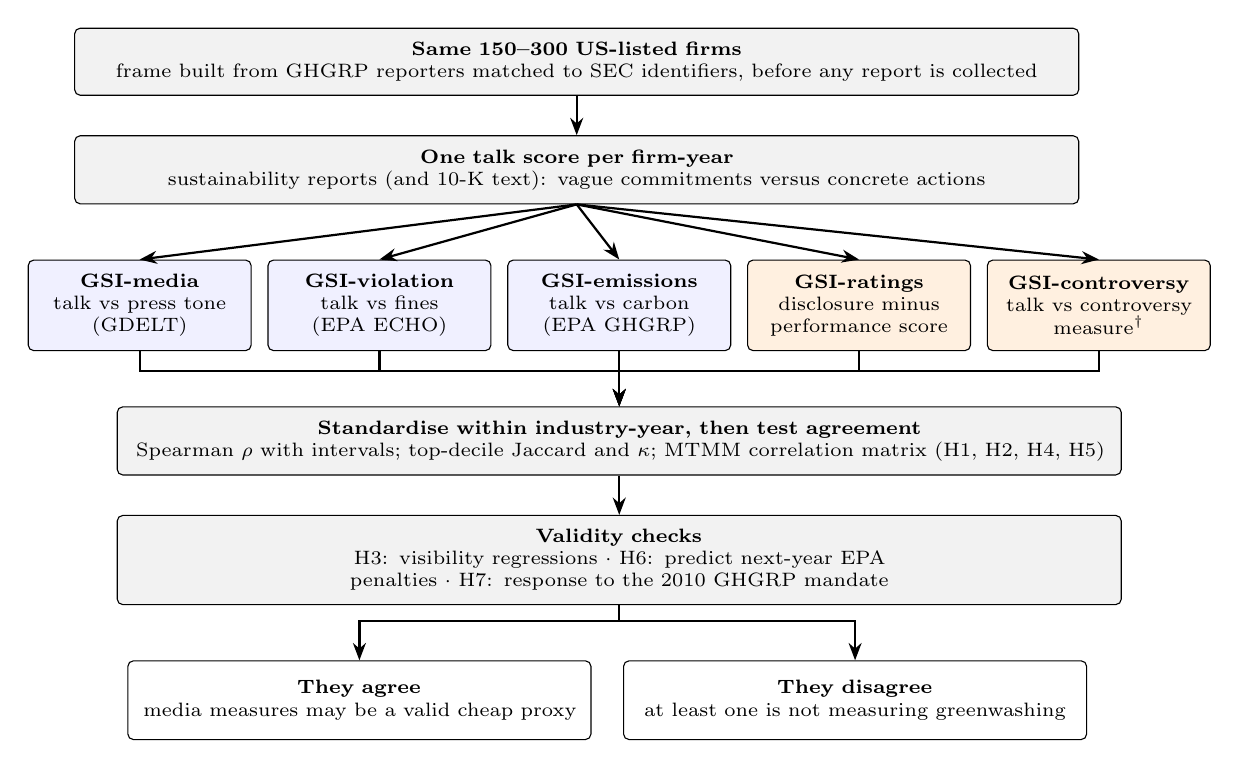
\begin{tikzpicture}[
  font=\scriptsize,
  node distance=0.45cm,
  box/.style={draw, rounded corners=2pt, align=center, inner sep=4pt, text width=2.55cm, minimum height=1.15cm, fill=blue!6},
  wide/.style={draw, rounded corners=2pt, align=center, inner sep=5pt, text width=12.4cm, fill=gray!10},
  outc/.style={draw, rounded corners=2pt, align=center, inner sep=4pt, text width=5.6cm, minimum height=1.0cm},
  arr/.style={-{Stealth[length=2.2mm]}, thick}
]
\node[wide] (frame) {\textbf{Same 150--300 US-listed firms}\\
 frame built from GHGRP reporters matched to SEC identifiers, before any report is collected};
\node[wide, below=0.5cm of frame] (talk) {\textbf{One talk score per firm-year}\\
 sustainability reports (and 10-K text): vague commitments versus concrete actions};
\node[box, below=0.7cm of talk, xshift=-5.55cm] (media) {\textbf{\GSI{media}}\\talk vs press tone\\(GDELT)};
\node[box, right=0.2cm of media] (viol) {\textbf{\GSI{violation}}\\talk vs fines\\(EPA ECHO)};
\node[box, right=0.2cm of viol] (emis) {\textbf{\GSI{emissions}}\\talk vs carbon\\(EPA GHGRP)};
\node[box, right=0.2cm of emis, fill=orange!12] (rat) {\textbf{\GSI{ratings}}\\disclosure minus\\performance score};
\node[box, right=0.2cm of rat, fill=orange!12] (con) {\textbf{\GSI{controversy}}\\talk vs controversy\\measure\dg};
\node[wide, below=0.7cm of emis] (std) {\textbf{Standardise within industry-year, then test agreement}\\
 Spearman $\rho$ with intervals; top-decile Jaccard and $\kappa$; MTMM correlation matrix (H1, H2, H4, H5)};
\node[wide, below=0.5cm of std] (val) {\textbf{Validity checks}\\
 H3: visibility regressions $\cdot$ H6: predict next-year EPA penalties $\cdot$ H7: response to the 2010 GHGRP mandate};
\node[outc, below=0.7cm of val, xshift=-3.3cm] (agree) {\textbf{They agree}\\media measures may be a valid cheap proxy};
\node[outc, right=0.4cm of agree] (dis) {\textbf{They disagree}\\at least one is not measuring greenwashing};
\draw[arr] (frame) -- (talk);
\foreach \n in {media,viol,emis,rat,con}{\draw[arr] (talk.south) -- (\n.north);}
\foreach \n in {media,viol,rat,con}{\draw[arr] (\n.south) -- ++(0,-0.25) -| (std.north);}
\draw[arr] (emis.south) -- (std.north);
\draw[arr] (std) -- (val);
\draw[arr] (val.south) -- ++(0,-0.2) -| (agree.north);
\draw[arr] (val.south) -- ++(0,-0.2) -| (dis.north);
\end{tikzpicture}
\caption{The proposed design. The two shaded indices (orange) are added after the extended
literature. Nothing in the figure has been computed.}
\label{fig:design}
\end{figure}

% ============================ 7. COMBINING ==================================
\section{Combining the papers: how we could get better results}
\label{sec:combining}

This section turns the 24 papers into twelve improvements to the design. Each is labelled
\emph{from a paper}, when the idea comes from a specific paper and we rely on that paper's own
result, or \emph{our proposal}, when it is ours, motivated by one or more papers but not tested by
them. None of this has been built.

\subsection{Compare five measures, not three}
\emph{From \citet{yu2020}, \citet{ghitti2024}; supported by \citet{luu2025}, \citet{liu2024},
\citet{bacher2025}.} Add the ratings-gap index and a controversy-based index to the three original
ones. These are what applied finance actually uses, so whether they agree with the hard anchors is
probably the most practically relevant result the study could give. The construction of the Ghitti
et al.\ measure is unverified.

\subsection{Use multi-trait multi-method logic}
\emph{Our proposal.} Treat greenwashing as one trait measured by several methods, the anchors.
Report the full correlation matrix of the five indices and ask whether indices that share an anchor
type (violations, emissions) correlate more with each other than with media-based ones. That turns
H4 into a standard validity test. As a reference point for ``moderate'' agreement we would use the
average correlation of about 0.45 between ESG raters reported by \citet{gibsonbrandon2021}\dg, once
confirmed from the paper.

\subsection{Test event responses}
\emph{From \citet{utz2019}\dg, \citet{cho2009} and Paper 2's difference-in-differences.} Use dated,
external events such as EPA formal enforcement actions and major penalties. A measure that
captures misconduct should move around them: the talk score rises after the event
\citep{gorovaia2025,cho2009}, the violation index rises by construction, and the media index rises
if media tracks conduct. A media index that moves with coverage spikes but not with enforcement
events is tracking attention, not conduct.

\subsection{Measure omission, not just tone}
\emph{Our proposal, from \citet{boiral2013} and \citet{wang2025}.} Boiral compared 116 negative news
events against 23 reports by hand and found that 90\% were left out. We would automate the idea:
for each firm-year, take negative-tone, environment-themed events from GDELT and check whether the
sustainability report mentions the issue. The resulting omission rate is a media-anchored version
of Wang et al.'s selective-disclosure component, measured against events that actually happened
rather than a list of required topics. It uses media for what happened and the report for what was
said, which is a better use of media than average tone. Whether an event is in the news at all still
depends on visibility.

\subsection{Separate attention from tone}
\emph{Our proposal, motivated by \citet{drempetic2020}\dg, \citet{gibsonbrandon2021}\dg\ and
\citet{raghunandan2022}.} Split media into coverage volume, average tone and the count of negative
events. Then build a visibility-adjusted media index: the residual from regressing media tone on log
size, log coverage volume and sector. If the adjusted index agrees with the hard anchors much better
than the raw one, that is direct evidence for H3 and a usable correction for practitioners.

\subsection{Define greenwashing as talk conditional on performance}
\emph{Our proposal, from \citet{clarkson2008}\dg\ and \citet{tadros2019} against Paper 2.} Good
performers can legitimately say more, so raw talk is ambiguous. For each anchor, regress the talk
score on that anchor's performance measure with sector-year effects and use the residual as the
greenwashing score: talk that the firm's actual performance does not explain. Each index then
becomes a principled ``talk minus what performance justifies'', rather than an arbitrary difference
of two differently scaled numbers.

\subsection{Use the published cheap-talk definition for the talk side}
\emph{From \citet{bingler2022,bingler2024}.} Adopt the cheap talk index definition (the share of
imprecise versus precise climate commitments\dg) rather than inventing a new promise-versus-action
score. It is validated, published and directly comparable to prior results. This is a design choice
for a possible future implementation; nothing is built in this project.

\subsection{Standardise peer-relatively}
\emph{From \citet{yu2020}\dg.} Standardise every index within industry-year before comparing, so
sector differences in emissions or newsworthiness do not drive agreement or disagreement. We have
this description of Yu et al.'s construction only from our brief; the description of the measure in
\citet{luu2025}, which we read, standardises over the sample and does not say within industry-year.

\subsection{Use predictive validity as the tie-breaker}
\emph{From \citet{liu2024}, \citet{ghitti2024}, \citet{bacher2025}; formalised as H6.} If the indices
disagree, the question becomes which to trust. Test which index best predicts future conduct
(next-year EPA penalties, and emissions growth as in \citealp{bingler2024}) and future market
outcomes (crash risk, firm value). Conduct outcomes come first, because market outcomes can
themselves reflect visibility.

\subsection{Use the GHGRP as a natural experiment}
\emph{From \citet{luu2025}; formalised as H7.} The GHGRP's 2010 start, with its 25,000 tonne
threshold, gives a before-and-after and a treated-and-untreated split. We check which indices
register the policy effect in the direction Luu et al.\ report. This reuses the data source we
already plan to use.

\subsection{Combine only after testing agreement}
\emph{Our proposal, building on \citet{dorfleitner2024}.} Their framework combines pillars into one
indicator. We add the step before: if the pillars do not agree, averaging them hides the
disagreement. So we (a) report agreement first; (b) build a ``consensus greenwasher'' flag, a firm in
the top decile on at least two hard anchors, as a conservative combined measure; and (c) only then
consider a weighted composite, with weights justified by predictive validity rather than the equal
weighting that Paper 1 uses without justification. Dorfleitner and Utz themselves suggest calibrating
weights on firm-years where case examination shows whether greenwashing occurred, which is close in
spirit to the tie-breaker above.

\subsection{Check whether Paper 1's formula problem is shared}
\emph{Our proposal, from \citet{lagasio2024}.} Compare Lagasio's ESGSI with the GSI of
\citet{davidescu2026}. If the ``severity index'' family generally scores report text without an
external term, our Paper 1 finding becomes a finding about a strand of the literature. We have
established one thing: Paper 1 does not cite Lagasio. Whether the ESGSI has an external term is an
open check that needs the full text of Lagasio's paper.
% ============================ 8. DATASETS ===================================
\section{Datasets and access}
\label{sec:data}

Everything proposed here uses free or open sources, apart from the optional ratings data. None of
these has been accessed. The rate limits and fields below come from the providers' documented
behaviour and need to be re-checked against the live documentation before any use.

\begin{table}[!htbp]
\centering
\caption{Data sources for a future implementation. None has been accessed.}
\label{tab:data}
\small
\begin{tabularx}{\textwidth}{@{}L{2.5cm}L{4.0cm}X@{}}
\toprule
\textbf{Source} & \textbf{What it gives us} & \textbf{Access and the catch}\\
\midrule
GDELT & Global news with a tone score per article; the media anchor & Free, no login. Returns about 250 articles per query through the web interface, so long histories need the bulk route. Company-name matching is noisy. Volume is confounded with size, so we keep it as a variable.\\
EPA ECHO & US facility inspections, violations and penalties; the violation anchor & Free, no key. Results are paginated and some fields cover a fixed multi-year window. Facilities are not companies, so aggregating to parent company is the central difficulty.\\
EPA GHGRP & Facility greenhouse gas emissions; the emissions anchor & Free download. Covers facilities emitting 25,000 tonnes of \co\ a year or more, Scope 1, US only. Publishes a parent-company field that helps entity matching.\\
SEC EDGAR & Filings, and the company identifier that ties everything together; 10-K text as a supplementary talk source & Free, but every request must carry a contact email, and requests are limited to ten per second.\\
Responsibility Reports & An archive of sustainability report PDFs & Free, no programmatic interface, so it needs scraping, after checking the site's terms. Coverage skews to large, prominent firms, which is why the sample frame is built first.\\
CDP & Standardised climate disclosures & Partly licensed; optional. Participation itself correlates with size and visibility.\\
Violation Tracker & Violations and penalties under federal laws, compiled by Good Jobs First; a cross-check on ECHO, used by \citet{raghunandan2022} & Not accessed. Its licence, bulk-download terms and parent-company coverage are all unverified.\\
\bottomrule
\end{tabularx}
\end{table}

The weakest link is the join, not any single source. The EPA tracks facilities, the stock market
tracks companies, and GDELT tracks names as they appear in news text, and none share an identifier.
We would work from the most reliable evidence downwards: the GHGRP parent-company field, then the
shared facility identifier to reach violations, then cleaned-name matching, then approximate
matches checked by hand. The match rate must be measured explicitly, because an unmeasured match
rate makes every downstream correlation uninterpretable.

% ============================ 9. THREATS ====================================
\section{Threats to validity and limitations of this review}
\label{sec:threats}

\subsection{Threats to the proposed design}

\begin{enumerate}
\item \lab{Entity-matching error} is the dominant risk. Bad company-to-facility links inject noise
  that biases correlations toward zero, which would look like support for our hypothesis for the
  wrong reason. A null result is interpretable only if the match rate is high and audited.
\item \lab{Sector confounding.} Heavy industry both emits more and attracts more negative coverage.
  Sector fixed effects and peer-relative standardisation address this.
\item \lab{Enforcement heterogeneity.} ECHO reflects regulator activity as well as firm conduct.
\item \lab{The GHGRP threshold} restricts and skews the sample frame toward industrial firms.
\item \lab{Reverse causality in media tone.} Coverage may follow a violation rather than detect
  greenwashing independently; lagged specifications are a reason to test.
\item \lab{Non-violation is not compliance.} A firm with no recorded violation is unpenalised, not
  proven clean \citep{gorovaia2025}.
\item \lab{Ratings-based indices inherit rating bias.} Both halves of a ratings gap are third-party
  scores, which rise with size and data availability \citep{drempetic2020}\dg\ and disagree across
  providers \citep{gibsonbrandon2021}\dg.
\end{enumerate}

\subsection{Limitations of this review}

\begin{itemize}
\item \lab{Fifteen of the nineteen new papers were read by abstract only.} Table~\ref{tab:basis}
  shows which. For four of those (Clarkson et al., Yu et al., Utz, and Drempetic et al.) neither
  Crossref nor OpenAlex had an abstract, so our description rests on our research brief and, for
  Yu et al., on how two papers we read describe it. A dagger (\dg) marks details taken from the
  brief and unconfirmed. We did not download the paywalled papers, or the open-access papers that
  publisher sites would not serve to a script. The 15 are listed with direct links in
  \texttt{papers/TO\_OBTAIN.md}.
\item \lab{The construction of the Ghitti et al.\ measure is unverified.} Our brief describes it as
  an ESG-score-minus-controversy-score gap; the abstract does not say so, and we could not read the
  method section. The same applies to the Bacher et al.\ use of that measure and to the Liu et al.\
  use of the Yu et al.\ measure. These are the first papers to fetch.
\item \lab{The selection of the 19 papers was not a systematic search.} They were assembled in
  research, not through a documented search protocol, so the review cannot claim to have covered
  the literature. This is why the refined gap keeps its hedge.
\item \lab{Citation checks.} All 24 citations were verified against Crossref. One DOI (Bingler et
  al.\ 2022) needed correcting, one publication date is flagged (Hrasky 2012, where Crossref's print
  date is 30 December 2011 for the 2012 volume), and pages were added for Ghitti et al. The
  record is in \texttt{papers/SOURCES.md}.
\item \lab{Paper 1's indexing.} \citet{davidescu2026} is peer-reviewed and indexed, but its
  journal is not credited on some national publication lists, and the problems we found in its
  formula are consistent with limited review scrutiny. We do not treat its index as validated.
\item \lab{Nothing has been measured.} Hypotheses H1--H7 and the twelve improvements are designs.
  No data has been collected, and no result in this report is our own empirical finding, with one
  exception: the arithmetic check of Paper 1's published aggregation rule in
  Table~\ref{tab:gsiverify}.
\end{itemize}

\begin{table}[!htbp]
\centering
\caption{What each of the 19 additional notes is based on.}
\label{tab:basis}
\small
\begin{tabularx}{\textwidth}{@{}L{4.2cm}X@{}}
\toprule
\textbf{Basis} & \textbf{Papers}\\
\midrule
Full text read & Bingler et al.\ 2022; Luu et al.; Dorfleitner and Utz; Raghunandan and Rajgopal\\
Abstract and metadata & Lagasio; Bingler et al.\ 2024; Hrasky; Tadros and Magnan; Cho et al.; Liu et al.; Boiral; Ghitti et al.; Bacher et al.; Cho 2009; Gibson Brandon et al.\\
Research brief and metadata only (no abstract available) & Clarkson et al.; Yu et al.; Utz; Drempetic et al.\\
\bottomrule
\end{tabularx}
\end{table}

% ============================ 10. CONCLUSION ================================
\section{Conclusion and next steps}
\label{sec:conclusion}

Reading 24 papers by reality anchor gives a clear picture. A talk--action gap shows up wherever it
has been tested against an outside fact, and quantity of disclosure is a poor proxy for honesty. At
the same time, three apparent contradictions (about mandatory disclosure, about who talks more, and
about large firms) look much less like contradictions once we see what each paper anchored its
measure to. Size and visibility appear to shape what gets measured, not only what firms do.

The gap, as far as we found, is a specific one: nobody has built several greenwashing indices on
the same firms, each anchored to a different reality check, and tested whether they rank the same
firms as worst. We have set out a design for that test with seven hypotheses and twelve
improvements, and we have said plainly where our evidence is thin.

\textbf{Next steps.} In order:
\begin{enumerate}
\item Fetch the papers in \texttt{papers/TO\_OBTAIN.md}, starting with Ghitti et al.\ and Bacher et
  al., to confirm the controversy measure, and with Lagasio, to settle the open check on Paper 1.
\item Confirm the details marked with a dagger from the papers themselves, in particular the
  rater-correlation figure of about 0.45 that we plan to use as a benchmark.
\item Build the firm list from GHGRP and SEC records and measure the entity-match rate before
  anything else. It is the step most likely to cause trouble.
\item Only then start with the news data, which needs no login and no facility matching, to get one
  complete path working.
\end{enumerate}
None of these steps has begun.

% ============================ BIBLIOGRAPHY ==================================
\bibliographystyle{plainnat}
\bibliography{references}

\end{document}
